%!TeXroot=。。/main。tex

\chapter{区块链上隐私保护技术}

在区块链系统的实际使用中,为了保证区块链上记录数据的可溯源、可验证等特性,所有数据都必须公开给区块链网络中的所有节点。这一特性在保障安全、可验证的同时,导致恶意攻击者可以直接获取区块链账本中记录的数据,并通过分析数据窥探用户隐私。攻击者通过分析区块链账本中记录的交易数据,发掘其中规律,将用户的不同地址、交易数据关联,并进一步对应到用户的现实身份[7-14]。这类分析攻击主要分为地址聚类和身份定位两阶段。地址聚类阶段根据用户行为特征将可能属于同一用户的地址、交易进行聚类,得到地址间关联关系。身份定位阶段搜集与区块链地址相关联的用户信息,例如论坛、交易所等服务记录的与链上地址对应的手机、邮箱、IP地址等用户链下信息,再根据搜集到的信息确定用户身份,关联该用户所有地址与交易信息,揭露该用户的所有历史记录。

近年来,许多研究者开始关注区块链系统中的隐私问题,该领域中相应的防御技术也不断出现。在区块链隐私分析上,祝烈煌等人从身份隐私和交易隐私两方面分析区块链中的隐私问题,身份隐私指用户身份信息和区块链地址之间的关联关系,交易隐私指区块链中存储的交易记录及背后的知识。Sarah等人提出用抗追溯性来度量区块链中用户信息的匿名性。本文从账本存储和网络通信两个方面,分析区块链系统中隐私信息可能泄露的内容和方式。从账本存储角度,需要保护用户存储在区块链账本上的数据记录所包含的隐私信息;从网络通信角度,需要保护区块链网络中的节点隐私及网络通信中的流量等隐私信息。在隐私保护技术方面,祝烈煌等人[30]从网络层、交易层和应用层出发分别描述区块链隐私保护面临的威胁以及采用的保护技术。Merve等人和李旭东等人将研究分为两大类:基于比特币系统的研究和针对比特币系统进行拓展和替换的研究。

本章对比特币系统以外的区块链隐私保护技术进行更大范围的技术介绍与对比。主要通过技术实现原理,将保护技术划分为地址混淆,信息隐藏和通道隔离,并对各类技术抽象出通用模型,然后介绍各类隐私保护技术的实现及对比。其中地址混淆机制通过交易交换不同用户的资产,对同一用户不同地址间的关联关系进行混淆,从而破坏地址聚类的假设前提;信息隐藏机制通过零知识证明、同态加密等密码学技术加密区块链账本中记录的隐私信息,同时保持账本正确性的可验证;通道隔离机制在区块链网络中设置访问权限,将需要权限访问的数据保护在特定通道中。

\section{区块链隐私及威胁}

传统的区块链系统中通常采用假名机制和广播机制保护用户隐私。其中假名机制指用户可以独立生成任意数量的区块链地址,不需要通过注册或者认证机制。同一用户生成的不同地址可以单独使用,彼此间不存在任何关联关系。因此,仅通过区块链地址无法关联到用户的真实身份,该机制能隔离用户在区块链上不同操作的记录。广播机制指区块链系统通过p2p网络传输数据,网络中采用洪水广播协议传播消息,接受节点无法判断消息来源是消息的直接发起者还是转发者,从而保护消息真实发起者的身份。
假名机制和广播机制能在一定程度上保护区块链用户的隐私安全。但在实际应用中,用户隐私仍面临各类威胁,主要存在于记录数据的分布式账本和区块链去中心化网络中各节点的相关信息。为了保证去中心化系统的正确性和安全性,区块链系统中的所有节点共同维护一致的分布式账本,记录区块链系统中的所有历史数据,用于验证用户提交的新事务的合法性。为了所有节点都能验证账本的正确性,账本中所有数据保持公开,因此账本数据能被攻击者轻易获取,攻击者通过分析公开账本中的记录严重威胁用户隐私。此外,区块链系统采用去中心化网路进行通信,在非许可链系统中,节点加入网络不需要任何身份认证,这在增强了扩展性的同时也导致攻击者可以自由部署节点加入网络,监听网络中各节点隐私信息以及网络中通信信息。本章围绕这两部分介绍需要保护的隐私内容及对应的威胁方式。

\subsection{账本隐私及威胁}

区块链账本记录了区块链系统中的各类事务数据,由于目前区块链系统主要应用于密码货币领域,因此区块链账本主要记录交易数据。交易模型主要分为未花费交易输出(UTXO,UnspentTransactionOutput)模型和账户(Account)模型两类[34]。部分攻击方式针对特定的交易模型,例如交易网络构造攻击和资产追踪攻击针对UTXO模型。账本隐私主要包含以下内容:
交易内容隐私:账本记录的单笔交易内容,包含交易发起方、交易接受方、交易金额以及附带数据等隐私信息。
账户地址隐私:区块链地址与交易的关联关系,包含账户地址的交易记录、账户余额以及不同账户地址间交易关联等隐私信息。
用户身份隐私:用户和区块链地址、交易的关联关系,包含同一用户的交易记录、资金余额等隐私信息。
在区块链系统的实际应用中,用户常需要发起多输入交易,即存在多个输入资产的交易。该交易需要每个输入地址的签名,可以由一个或多个用户生成。由于多个用户对同一交易进行签名的过程较为复杂,通常多输入交易由同一用户生成。此外,在基于UTXO模型的交易系统中,未花费资产只能使用一次,因此当花费资产超过交易所需资产时,用户将超出部分的资产转移到自己的另一账户地址中。用于接受超出部分资产的账户地址通常称为找零地址。针对账本隐私包含的各类隐私,目前的主要攻击方式为账本分析攻击,通过分析区块链账本数据,利用用户常见的交易规律,构建账户地址与交易之间以及用户与账户地址之间的一对多对应关系,威胁账本地址隐私与用户身份隐私。攻击者根据区块链系统的设计与上述使用特征提出以下假设:

\begin{enumerate}
	\item 假设1 多输入交易的所有输入地址为同一用户所持有。
	\item 假设2 交易的找零地址和输入地址为同一用户所持有。
\end{enumerate}

2013年,Reid等人下载了比特币系统2009年1月3日至2011年7月12日的全部账本数据,通过分析数据首先构建交易网络。交易网络中节点表示单次交易,节点间的有向边为交易间的输出-输入对,表示前一次交易的输出作为后一次交易的输入,每条边同时记录了交易金额以及交易时间。

\begin{figure}
\centering
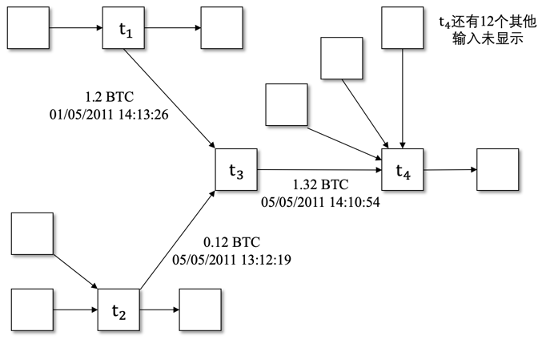
\includegraphics[width=11cm]{figures/sub-network.png}
\caption{交易网络示例}
\label{fig:framework}
\end{figure}

在交易网络的基础上,提取所有多输入交易,构建账户地址间的非完全网络,非完全网络中节点表示地址,节点间有向边表示地址间交易的时间和金额。Reid等人根据中本聪提到的多输入交易关联风险[1]提出假设1,即假设多输入交易的所有输入地址为同一用户所有。基于这一假设,在非完全网络的基础上,可以聚合属于同一用户的所有地址,进而构建用户网络,用户网络中节点表示一个用户,节点间的有向边表示用户间资产流动信息。

(a)Anexamplesub-networkfromtheincompletenetwork
(a)非完全网络中的局部示例

(b)Anexamplesub-networkfromtheusernetwork
(b)用户网络中的局部示例
Fig。2Examplesub-networksfromtheincompletenetworkandtheusernetwork[7]
图2非完全网络与用户网络示例[7]
	2013年,Androulaki等人[8]根据区块链钱包的应用特征提出了挖掘找零地址的方法,如果一个交易拥有两个输出,其中一个为已出现过的地址,另一个为新地址,则将新地址视为找零地址,并提出了假设2,即交易的找零地址和输入地址为同一用户所持有。为了验证假设的正确性,Androulaki等人在大学中构建了模拟的密码货币使用环境,通过搜集用户使用记录,并利用假设1和假设2进行分析,挖掘出40\%左右用户的真实身份。受此启发,Meiklejohn等人[9]给出了“找零地址”更完善的定义:
	找零地址如果交易t中的一个输出公钥地址pk满足以下所有特征,则可将pk视为“找零地址”。
1。	,该地址pk在非完全网络中入度为1,即在区块链账本中首次出现。
2。	交易t为铸币交易以外的普通交易。铸币交易即生成新区块时发布奖励的交易。
3。	不存在且,即不存在“自找零地址”。
4。	不存在,且,即pk为输出地址中唯一首次出现的地址。
综上所述,账本隐私内容主要集中于单次交易的内容及隐藏在多个相关交易之后的用户身份、账户余额等隐私信息。这部分信息记录在公开的区块链账本中,攻击者可以通过分析账本挖掘出其中的关联信息,威胁用户的账本隐私。

\subsection{网络隐私及威胁}

区块链系统通过去中心化的P2P网络进行节点间通信,而在非许可链系统中的网络不存在准入限制,这在增强了扩展性的同时也带来了潜在的风险。攻击者可以任意部署节点,监听网络中各节点隐私信息以及网络通信信息,甚至尝试对正常节点发起攻击。区块链网络主要存在以下隐私内容:

节点隐私:节点自身的隐私内容,包含节点网络IP、软件版本、服务器系统等隐私信息。
通信隐私:节点间通信隐私内容,包含节点间通信的数据内容以及通信流量情况。

2013年,Reid等人尝试利用BitcoinFaucet公开的区块链地址及IP地址对应关系进行分析,揭露比特币用户与实际物理位置的对应关系,该尝试只涉及到很少的节点。Bitnodes网站通过部署大量节点,探测全球范围内的比特币节点信息,其中IP地址分布信息如图3所示(截图于2019年08月01日)。

图3Bitnodes网站在世界范围内发现的比特币节点分布情况

探测攻击严重威胁节点隐私,更进一步,攻击者通过大量探测可以将区块链中广播的数据与实际发起节点关联,尽管区块链网络采用洪水广播的方式保护实际发起人,但是在布置大量探测节点后,攻击者有很大概率找出消息的真实发起节点。2011年,Kaminsky在黑帽大会上提出假设,假设第一次接受到消息时的来源节点即为该消息的真实发起节点。

(a)模式1单一转发者(b)模式2多转发者,无重复转发者


(c)模式3A多转发者,单一重复转发者(d)模式3B多转发者,多重复转发者
Fig。4Fourmessagepropagationmodes
图4四种消息传播模式

2014年,Koshy等人在Kaminsky所提出假设的基础上进行了完善,归纳一段时间内监听到的消息传播情况,提出了区块链网络中消息传播的四种模式(如图4所示)以及对应的真实发起者假设。这一攻击方式通过监听消息传播模式,分析真实发起节点,将IP地址与消息中包含的链上地址对应,威胁通信隐私与用户身份隐私。

模式1单一转发者该模式中消息只有一个节点重复发送。在广播协议中这种情况并不常见,通常出现原因在于该节点发送不合法消息,其他节点拒绝转发该消息。因此可以假设该节点为消息实际发送者。
模式2多转发者,无重复转发者该模式中有多个节点参与消息的转发,每个节点只发送一次。这种模式是网络中最常见的消息传播模式,在Koshy等人收集的数据中占据91。4%。该模式中假设第一次接受到的消息发起者为消息的真实发起者。
模式3A多转发者,单一重复转发者该模式中有多个节点参与消息的转发,除了一个节点重复多次外,其他节点只发送一次。该模式中,假设唯一的重复转发者为消息的真实发起者。
模式3B多转发者,多重复转发者

该模式中有多个节点参与消息的转发,多个节点重复发送,该模式中难以推断实际发起节点,并且所占比例较小,为2。8\%,因此Koshy等人放弃了这部分数据。

综上所述,区块链系统的隐私内容以及对应的攻击方式总结如表2所示。

Table2PrivacyInformationandThreatinBlockchain
表2区块链隐私内容及对应攻击方式

区块链隐私分类	隐私保护内容	隐私威胁攻击方式
交易内容隐私	账本记录的单笔交易信息,包含
交易发起方、交易接受方、交易
金额以及附带数据等隐私信息	通过区块链钱包、浏览器等
工具爬取区块链账本记录
账户地址隐私	区块链地址与交易的关联关系,包
含账户地址的交易记录、余额以及
不同账户间交易等隐私信息	通过分析区块链账本记录,
构建交易网络
用户身份隐私	用户和区块链地址、交易的关联关系,包含同一用户的交易记录、资金余额等隐私信息	利用区块链交易特征,在交易网
络的基础上构建用户网络。也从
论坛、交易所等区块链服务获取
节点隐私	节点相关信息,包含节点网络IP、
软件版本、服务器系统等隐私信息	在区块链网络中部署节点监听
或爬取其他公开信息获取
通信隐私	节点间通信内容,包含节点间通
信的数据内容以及通信流量情况	通过在区块链网络中部署监听节
点,监听节点间通信进行获取

\section{地址混淆机制}

\subsection{中心化混币}

\subsection{去中心化混币}

\section{信息隐藏机制}

\subsection{账本信息隐藏}

\subsection{网络信息隐藏}

\section{通道隔离机制}

\subsection{链下通道隔离}

\subsection{多链通道隔离}

